\documentclass[tikz, crop, border=0pt]{standalone}
% class=minimal, convert
%\usepackage{tikz}

\usepackage[utf8x]{inputenc}
\usepackage[T1]{fontenc}
\usepackage{lmodern}
\usepackage{textcomp}

\usetikzlibrary{arrows.meta, backgrounds}

\tikzset{%
    curve/.style={thick, color=red},
    leftpoint/.style={color=black},
    rightpoint/.style={color=white, draw=black},
    %my thick box/.style={thick,color=blue}
}

\begin{document}
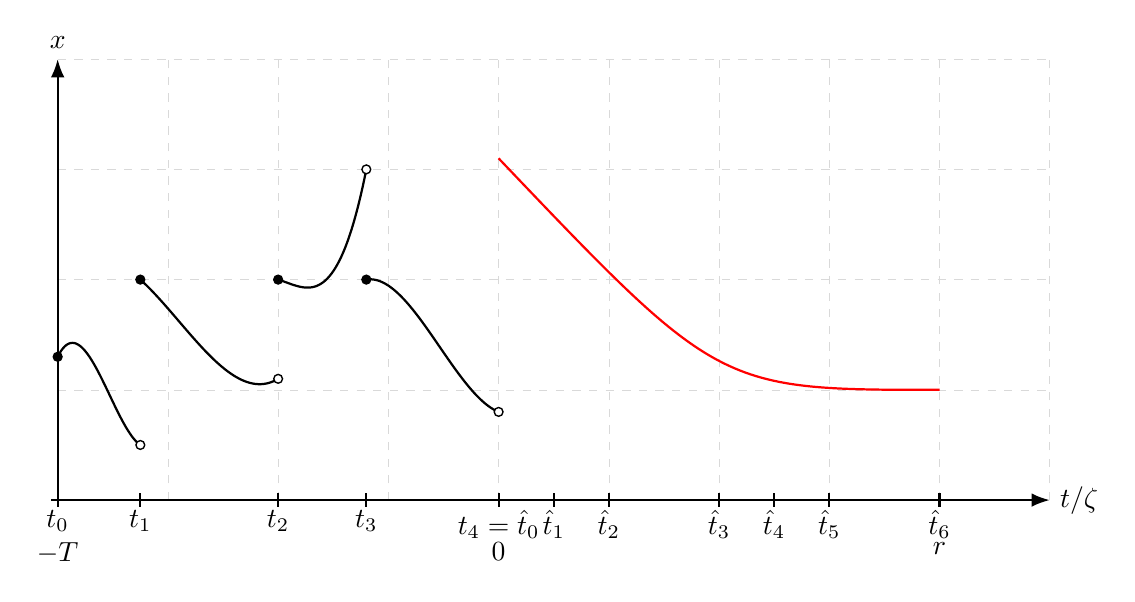
\begin{tikzpicture}[line width=0.5pt, scale=1.4, >=Latex]

	% grid
	\draw[help lines, color=gray!30, dashed] (-4,0) grid (5,4);
	
	% time axis
	\draw[->, thick] (-4.06,0) -- (5,0) node[right] {$t/\zeta$};
	\draw[->, thick] (-4,-0.06) -- (-4,4) node[above] {$x$};

	% ticks
	\draw (-4,0) node[below] {$t_0$};
	\draw (-4,-0.3) node[below] {$-T$};
	\draw[thick] (-4,-0.06) -- (-4,0.06);
	\draw (-3.25,0) node[below] {$t_1$};
	\draw[thick] (-3.25,-0.06) -- (-3.25,0.06);
	\draw (-2,0) node[below] {$t_2$};
	\draw[thick] (-2,-0.06) -- (-2,0.06);
	\draw (-1.2,0) node[below] {$t_3$};
	\draw[thick] (-1.2,-0.06) -- (-1.2,0.06);
	\draw (0,0) node[below] {$t_4=\hat t_0$};
	\draw (0,-0.3) node[below] {$0$};
	\draw[thick] (0,-0.06) -- (0,0.06);

	\draw (0.5,0) node[below] {$\hat t_1$};
	\draw[thick] (0.5,-0.06) -- (0.5,0.06);
	\draw (1,0) node[below] {$\hat t_2$};
	\draw[thick] (1,-0.06) -- (1,0.06);
	\draw (2,0) node[below] {$\hat t_3$};
	\draw[thick] (2,-0.06) -- (2,0.06);
	\draw (2.5,0) node[below] {$\hat t_4$};
	\draw[thick] (2.5,-0.06) -- (2.5,0.06);
	\draw (3,0) node[below] {$\hat t_5$};
	\draw[thick] (3,-0.06) -- (3,0.06);
	\draw (4,0) node[below] {$\hat t_6$};
	\draw (4,-0.3) node[below] {$r$};
	\draw[thick] (4,-0.06) -- (4,0.06);
	%\draw[thick] (\x,-0.06) -- (\x,0.06);
	
	% initial condition
	%\draw[curve] (-4,1.3) .. controls (-3.5,2) and (-3.5,0.5) .. (-3.25,0.5);
	\newcommand{\ta}{-4}
	\newcommand{\tb}{-3.25}
	\newcommand{\ca}{1.3}
	\newcommand{\cb}{1.5}
	\newcommand{\cc}{-4.9}
	\newcommand{\cd}{2.6}
	\draw[thick] plot[samples=50, smooth, domain=\ta:\tb] (\x, {\ca+\cb*((\x-\ta)/(\tb-\ta))+\cc*((\x-\ta)/(\tb-\ta))^2+\cd*((\x-\ta)/(\tb-\ta))^3});
	\filldraw[leftpoint] (-4,1.3) circle (0.04);
	\filldraw[rightpoint] (-3.25,0.5) circle (0.04);

	%\draw[curve] (-3.25,2) .. controls (-2.75,1.5) and (-2.75,0.6) .. (-2,1.1);
	\renewcommand{\ta}{-3.25}
	\renewcommand{\tb}{-2.0}
	\renewcommand{\ca}{2.0}
	\renewcommand{\cb}{-1.125}
	\renewcommand{\cc}{-1.2}
	\renewcommand{\cd}{1.425}
	\draw[thick] plot[samples=50, smooth, domain=\ta:\tb] (\x, {\ca+\cb*((\x-\ta)/(\tb-\ta))+\cc*((\x-\ta)/(\tb-\ta))^2+\cd*((\x-\ta)/(\tb-\ta))^3});
	\filldraw[leftpoint] (-3.25,2) circle (0.04);
	\filldraw[rightpoint] (-2,1.1) circle (0.04);
	
	%\draw[curve] (-2,2) .. controls (-1.5,2) and (-1.3,2.5) .. (-1.2,3);
	\renewcommand{\ta}{-2.0}
	\renewcommand{\tb}{-1.2}
	\renewcommand{\ca}{2.0}
	\renewcommand{\cb}{-0.24}
	\renewcommand{\cc}{-0.52}
	\renewcommand{\cd}{1.76}
	\draw[thick] plot[samples=50, smooth, domain=\ta:\tb] (\x, {\ca+\cb*((\x-\ta)/(\tb-\ta))+\cc*((\x-\ta)/(\tb-\ta))^2+\cd*((\x-\ta)/(\tb-\ta))^3});
	\filldraw[leftpoint] (-2,2) circle (0.04);
	\filldraw[rightpoint] (-1.2,3) circle (0.04);
	
	%\draw[curve] (-1.2,2) .. controls (-0.5,2) and (-0.5,1) .. (0,0.8);
	\renewcommand{\ta}{-1.2}
	\renewcommand{\tb}{0.0}
	\renewcommand{\ca}{2.0}
	\renewcommand{\cb}{0.2}
	\renewcommand{\cc}{-3.52}
	\renewcommand{\cd}{2.12}
	\draw[thick] plot[samples=50, smooth, domain=\ta:\tb] (\x, {\ca+\cb*((\x-\ta)/(\tb-\ta))+\cc*((\x-\ta)/(\tb-\ta))^2+\cd*((\x-\ta)/(\tb-\ta))^3});
	\filldraw[leftpoint] (-1.2,2) circle (0.04);
	\filldraw[rightpoint] (0,0.8) circle (0.04);

	% term value
	\draw[curve] (0,3.1) .. controls (2,1) and (2,1) .. (4,1);

% A=[1 0 0 0; 1 1 1 1; 0 1 0 0; 0 1 2 3]
% t0=-3.25; t1=-2.0;
% b=[2.0,1.1,-0.75,0.75]
% coeff=A\b


	%\draw[thick, domain=-5:0, samples=50] plot (\x, {-1.5*sqrt(pow(\x,2))*sin(\x r)/(\x-3)+cos(\x r)});


	

	

	

\end{tikzpicture}
\end{document}